\DiaryEntry{Divisibility}{2018-08-28}{Maths}


Based on \href{https://exupero.org/hazard/post/prime-modulo/}{this article}. The article deals with (graphical) helpers to determine the divisibility of numbers $n$ by primes. The numbers are presented by their digits; (different to the article), we have

\bee
n = n_1 + 10 n_2 + 100 n_3 + \cdots + 10^N c_N
\eee


\paragraph{Divisibility by 7.} In order to check whether a number is divisible by 7, the article uses the following Figure.

\begin{figure}[H]
	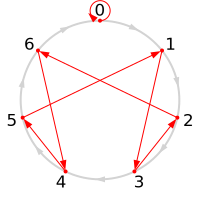
\includegraphics[scale=1.5]{images/divisibility_7.png}
\end{figure}

The procedure is as follows:

\begin{itemize}
	\item Start at zero.
	\item Take the leftmost digit ($c_N$) and go along the circle $c_N$ steps in clock-wise direction.
	\item Follow the red arrow to another point.
	\item Repeat from step $2$ with $c_{N-1}$.
	\item If there are no digits left, the current position equals $n \bmod 7$.
\end{itemize}

As an example consider $n = 238$: We start at point zero and move two steps to $2$. Follow the red arrow to $6$. Move three steps to $2$. Follow the red arrow to $6$ and finally move eight steps. We arrive at zero as $238 / 7 = 34$.

This works basically as follows: The red arrows point from $i$ to $10i \bmod 7$. We start with the "most important" digit and by following the red arrow we obtain modulo-7. The we continue with the next smaller digit and so till we went through all digits, giving the remainder.


\paragraph{Divisibility by 13.} In a similar spirit, we can change the Figure to allow checking the divisibility by 13:

\begin{figure}[H]
	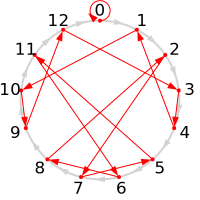
\includegraphics[scale=1.5]{images/divisibility_13.png}
\end{figure}

The rules are the same as above. As an example consider $n=169$: Start at zero, go one step to $1$ and follow the red arrow to $10$. Now move $6$ steps to $3$ and the red arrow brings us to $4$. Moving $9$ steps we arrive at zero as $169 / 13 = 13$.